\documentclass[a4paper, 12pt]{article}
\usepackage[total={17cm,25cm}, top=2.5cm, left=2.5cm, right=2.5cm,  includefoot]{geometry}
\usepackage[utf8]{inputenc}
\usepackage{array}
\usepackage{multirow}
\usepackage{hhline}
\usepackage{gensymb}
\usepackage{graphicx}
\graphicspath{ {} }
\usepackage[czech]{babel}
\usepackage{enumitem}
\usepackage{pdfpages}
\usepackage{amsmath}
\usepackage{verbatim}
\usepackage{listings}
\usepackage{hyperref}
\usepackage{amssymb}


\pagestyle{empty} % vypne číslování stránek




\usepackage[OT2,OT1]{fontenc}
\newcommand\cyr
{
\renewcommand\rmdefault{wncyr}
\renewcommand\sfdefault{wncyss}
\renewcommand\encodingdefault{OT2}
\normalfont
\selectfont
}
\DeclareTextFontCommand{\textcyr}{\cyr}
\def\cprime{\char"7E }
\def\cdprime{\char"7F }
\def\eoborotnoye{\char’013}
\def\Eoborotnoye{\char’003}
\setlength{\parindent}{1em} 
%\setlength{\parskip}{0.5ex}


\begin{document}

\begin{titlepage}
\begin{center}
\Huge
\vspace*{4.5cm}
Algoritmy v digitální kartografii \\
\vspace{0.2cm}

\Large  
Konvexní obálky\\
\vspace{0.2cm}

\normalsize  
Zimní semestr 2018/2019\\
%(oprava: )
\vspace{14cm}
\end{center}

\begin{flushright}
\Large
Tereza Kulovaná \\
Markéta Pecenová \\
\end{flushright}

\end{titlepage}


\pagestyle{plain}     % zapne obyčejné číslování
\setcounter{page}{1}  % nastaví čítač stránek znovu od jedné

\tableofcontents
\newpage

\section{Zadání}
Zadání úlohy bylo staženo ze stránek předmětu \href{https://web.natur.cuni.cz/~bayertom/index.php/teaching/algoritmy-v-digitalni-kartografii}{155ADKG}.

\begin{figure}[h!]
	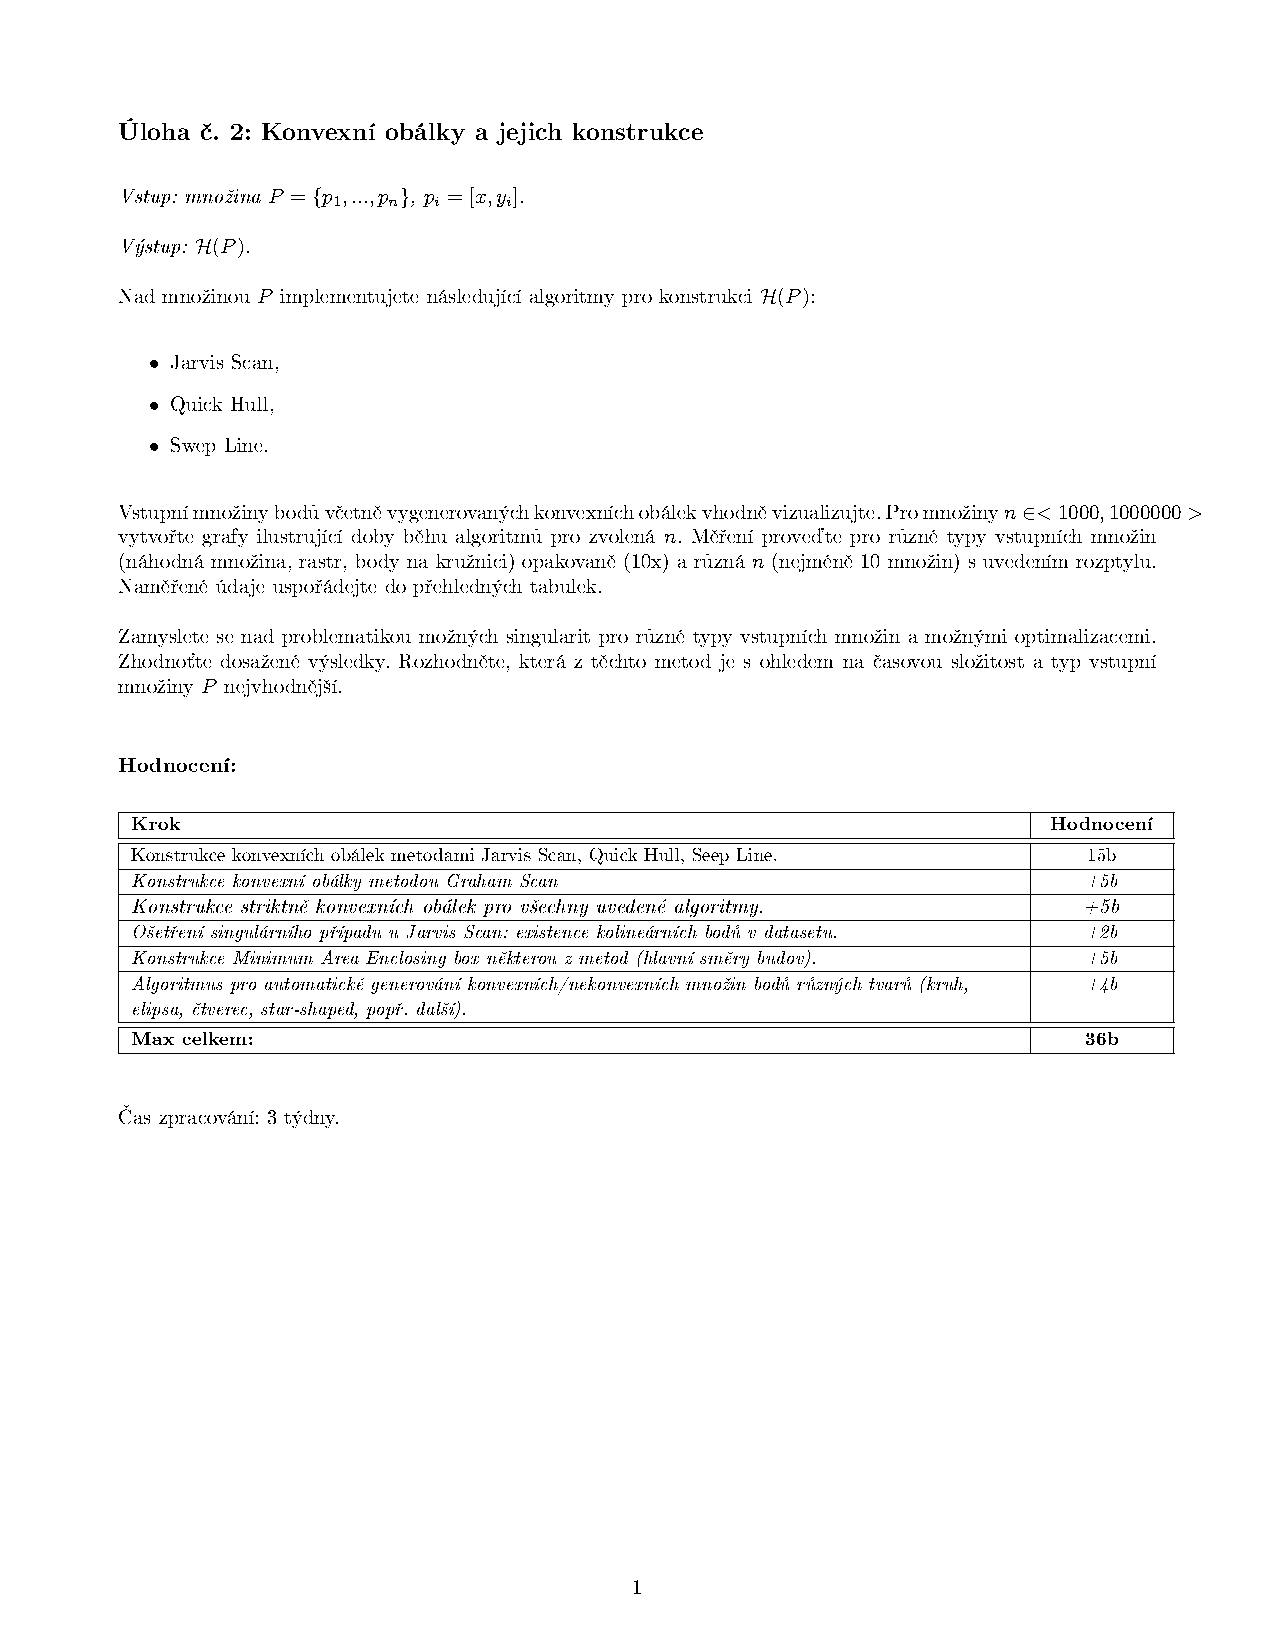
\includegraphics[clip, trim=0cm 10cm 0cm 3cm, width=1.0\textwidth]{./pictures/zadani02.pdf}
\end{figure}

V rámci této úlohy byly implementovány bonusové úlohy č. xx.
\clearpage

\section{Popis a rozbor problému}
Úloha \textbf{Konvexní obálky} se zabývá vytvořením aplikace, která nad vybranou vstupní množinou $S$ vytvoří tzv. konvexní obálku. Konvexní obálka je nejmenší konvexní mnoho\-úhelník $C$ obsahující všechny body z množiny $S$. V rámci úlohy se testuje výpočetní rychlost použitých algoritmů při konstrukci obálek nad danými vstupními množinami bodů. 

Své využití konvexní obálky nalézají v mnoha oborech. V kartografii se hojně využívají při detekci tvarů a natočení budov pro tvorbu minimálních ohraničujících obdélníků (???). Dále jsou vhodné pro analýzu tvarů či shluků. Konvexní obálky lze sestrojit v libovolném $\mathbb{R}^n$ prostoru, avšak pro účely této úlohy byl uvažován pouze prostor $\mathbb{R}^2$.

\begin{figure}[h!]
	\centering
	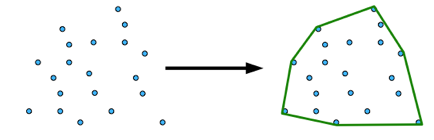
\includegraphics[width=13cm]{./pictures/ch.png}
	\caption{Ukázka konvexní obálky (\href{http://mind.cs.byu.edu/courses/312/projects/project2_files/ConvexHull_python.php}{\textsl{zdroj}})}
\end{figure}

Vzniklá aplikace k tvorbě konvexní obálek využívá čtyř výpočetních algoritmů: \textit{Jarvis Scan}, \textit{Quick Hull}, \textit{Sweep Line} a \textit{Graham Scan}. Čtvrtý z uvedených algoritmů patří mezi bonusové úlohy, které bylo možno implementovat.

\section{Algoritmy}
Tato kapitola se zabývá popisem algoritmů, které byly v aplikaci implementovány. 

\subsection{Jarvis Scan}
Prvním zvoleným algoritmem je \textit{Jarvis Scan}. Způsob, jakým vytváří konvexní obálku, nápadně připomíná balení dárků (proto je též občas nazýván jako \textit{Gift Wrapping Algorithm}). Mezi nevýhody tohoto algoritmu patří nutnost předzpracování dat a nalezení tzv. pivotu. Algoritmus dále není vhodný pro velké množiny bodů a ve vstupní množině $S$ nesmí být žádné tři body kolineární. Časová náročnost algoritmu je až $O(n^2)$, jeho výhodou však je velmi snadná implementace. \\

Mějme množinu bodů $S$ a pivota $q \in S$, jehož souřadnice Y je minimální ze všech bodů, a přidejme ho do konvexní obálky $H$. Následně do $H$ přidejme takový bod, který s posledními dvěma body přidanými do konvexní obálky svírá maximální úhel. Na začátku výpočtu je nutno inicializovat pomocný bod $s$, jehož souřadnice X je minimální a Y shodná s pivotem $q$, který zajistí dostatečný počet bodů pro výpočet prvního úhlu. Algoritmus končí ve chvíli, kdy nově přidaným bodem do konvexní obálky $H$ je opět pivot $q$. \\

Zjednodušený zápis algoritmu lze zapsat způsobem uvedeným níže:

\begin{enumerate}
\item Nalezení pivota $q$: $q$ = min($y$) 
\item Inicializace pomocného bodu $s$: $s$ = [min($x$), min($y$)]
\item Proveď: $q \in H$
\item Inicializace: $p_{j-1} = s$, $p_j = q$
\item opakuj kroky I–III, dokud $p_{j+1} \neq q$:
\begin{enumerate}[label=\Roman*.]
\item 	Najdi $p_{j+1}$: $\sphericalangle p_{j-1}, p_j, p_{j+1}$ = max
\item 	Proveď: $p_{j+1} \in H$
\item 	Přeindexuj: $p_{j-1} = p_j$, $p_j = p_{j+1}$
\end{enumerate}
\end{enumerate}


Singularity!!!!

\subsection{Quick Hull}
Druhý algoritmus použitý v aplikaci je \textit{Quick Hull}, který k výpočtu konvexní obálky využívá strategii \textit{Divide and Conquer}. Hlavní výhodou algoritmu je jeho rychlost, která není ovlivňována velkým počtem rekurzivních kroků, jak tomu bývá u jiných algoritmů. Časová náročnost výpočtu bývá v nejhorším případě $O(n^2)$ a nastává tehdy, pokud všechny body množiny $S$ náleží konvexní obálce $H$.\\

Mějme body $q_1$, resp. $q_3$, jejichž souřadnice X je minimální, resp. maximální ze všech bodů z množiny $S$. Veďme těmito body pomyslnou přímku, která prostor rozdělí na horní ($S_U$) a dolní ($S_L$) polorovinu. Zbylé body množiny $S$ roztřídíme do daných polorovin podle jejich pozice od přímky. V polorovině následně hledáme bod, který je od dané přímky nejvzdálenější, přidáme ho do konvexní obálky dané poloroviny a přímkami spojíme bod s krajními body přímky předchozí. Proces opakujeme, dokud od nově vzniklých přímek již neexistují vhodné body. Na závěr do konvexní obálky $H$ přidáme bod $q_3$, body konvexní obálky $H_U$ z poloroviny $S_U$, bod $q_1$ a nakonec body konvexní obálky $H_L$ poloroviny $S_L$. Do konvexní obálky $H$ je důležité přidávat body v tomto pořadí, jinak by došlo k nesprávnému vykreslení konvexní obálky $H$. \\

Algoritmus \textit{Quick Hull} se skládá z globální a lokální procedury. Globální část zahrnuje rozdělení množiny na dvě poloroviny a spojení již nalezených bodů konvexních obálek polorovin do jediné $H$. V lokální části se rekurzivně volá metoda, která hledá nejvzdálenější body od přímky v dané polorovině a přidává je do konvexní obálky dané poloroviny $H_i$.\\

Mezi singularity!!!\\

\textbf{Globální procedura}:
\begin{enumerate}
\item Inicializace: $H = \emptyset$, $S_U = \emptyset$, $S_L = \emptyset$ 
\item Nalezení $q_1$ = min($x$), $q_3$ = max($x$)
\item Proveď: $q_1 \in S_U$, $q_3 \in S_U$, $q_1 \in S_L$, $q_3 \in S_L$
\item Potupně pro všechna $p_i \in S$:
\subitem Podmínka ($p_i$ je vlevo od $q_1$, $q_3$) $\rightarrow S_U$
\subitem Jinak $ p_i \rightarrow S_L$
\item Proveď: $q_3 \in H$
\item Lokální procedura pro $S_U$
\item Proveď: $q_1 \in H$
\item Lokální procedura pro $S_U$
\end{enumerate}
~\\
\textbf{Lokální procedura nad polorovinou $S_i$}:
\begin{enumerate}[label=\Roman*.]
\item Pro všechny $p_i \in S_i$ kromě bodů přímky:
\subitem Podmínka ($p_i$ vpravo) $\rightarrow$ vzdálenost $d_i$
\subsubitem Podmínka ($d_i > d_{max}$) $\rightarrow d_{max} = d_i$, $p_{max} = p_i$
\item Podmínka (bod $p_{max}$ $\exists$) 
\subitem opakuj krok I. nad první nově vzniklou přímku
\subitem $p_{max} \in H_i$
\subitem opakuj krok I. nad druhou nově vzniklou přímku
\end{enumerate}

\subsection{Sweep Line}
Algoritmus \textit{Sweep Line} neboli \textit{Metoda zametací přímky} je dalším z algoritmů, které byly pro vytváření konvexních obálek implementovány. Jeho princip je založen na imaginární přímce, která se postupně přesouvá zleva doprava nad všem body množiny $S$. Body, které \uv{přejede}, přidá do dočasné konvexní obálky \={H}, která je následně upravena, aby byla konvexní. Pro tento algoritmus je opět nutné předzpracování vstupních dat (seřadit body $\in S$ podle souřadnice X) s náročností $O(n.$log$(n))$. Další nevýhodou je citlivost algoritmu na singularity, konkrétně na duplicitní body. Ty je vhodné během předzpracování odstranit.\\ 

Algoritmus je postaven na znalosti pozice již vyhodnocených bodů vůči nově přidá\-vanému bodu ukládáním jejich indexů do proměnných $p$ (předchůdce) a $n$ (následník). Zároveň je pro správné fungování algoritmu nutné dodržovat CCW orientaci (proti směru hodinových ručiček). Algoritmus má celkem tři fáze: iniciální a dvě iterativní.\\

V první fázi seřadíme body $p_i$ z množiny $S$ vzestupně podle souřadnice X. Následně z prvních dvou bodů vytvoříme přímku, jejíž koncové body umístíme do konvexní obálky $H$ a indexy bodů umístíme do $n$ a $p$. V první iterativní fázi vyhodnotíme, zda další přidávaný bod leží v horní či dolní polorovině v závislosti na jeho souřadnici Y vzhledem k předchozímu bodu, a opět obousměrně vyhodnotíme indexy $n$ a $p$. Ve druhé iterativní fázi opravujeme dočasnou konvexní obálku \={H} na konvexní $H$ vložením horních a dolních tečen a vynecháním nekonvexních vrcholů.\\

Zjednodušený zápis algoritmu: 
\begin{enumerate}
\item Seřazení $p_i$ podle souřadnice X
\item Pro body $p_0$, $p_1$ proveď:
\subitem $n$[0] = 1, $n$[1] = 0
\subitem $p$[0] = 1, $p$[1] = 0
\item Pro všechna $p_i \in S$, $i > 1$ proveď:
\subitem Podmínka ($y_i > y_{i-1}$) $\rightarrow$ $S_U$: $p$[i] = i-1, $n$[i] = $n$[i-1]
\subitem Jinak $\rightarrow$ $S_L$: $n$[i] = i-1 $p$[i] = $p$[i-1]
\subitem Oprava indexů: $n$[$p$[i]] = i, $p$[$n$[i]] = i
\subitem Dokud $n$[$n$[i]] je vpravo od i, $n$[i]:
\subsubitem $p$[$n$[$n$[i]]] = i, $n$[i] = $n$[$n$[i]]
\subitem Dokud $p$[$p$[i]] je vlevo od i, $p$[i]:
\subsubitem $n$[$p$[$p$[i]]] = i, $p$[i] = $p$[$p$[i]]
\end{enumerate}
%%vypsání polygonu z nasledníku??

Singularity

\subsection{!Graham Scan}

\section{!Problematické situace}
V úloze bylo nutné ošetřit sigularity, zda bod $q$ neleží v hraně některého z polygonů či v jejich vrcholech. Pro vyřešení tohoto problému byla použita metoda \textit{getDistanceEdgeQ} třídy \textbf{Algorithms}, která porovnává vzdálenost dvou bodů $p_1$ a $p_2$ na přímce $p$ se sumou vzdáleností těchto bodů k danému bod $q$. Je-li rozdíl vzdáleností menší než mezní hodnota $\epsilon$, je bod $q$ vyhodnocen, že leží na přímce.\\

$\mid d_{p_1,p_2} - \sum(d_{p_1,q} + d_{q,p_2}) \mid  < \epsilon \rightarrow q$ náleží přímce $p$.

\section{!Vstupní data}
Aplikace požaduje dva druhy vstupních dat:

\begin{enumerate}
\item soubor daných polygonů
\item daný bod $q$
\end{enumerate}

Seznam bodů jednotlivých polygonů je uložen v textovém souboru polygon.txt. Pro vykreslení jednotlivých polygonů v aplikaci je nutno tento soubor do aplikace nahrát pomocí tlačítka \textit{Load}. K vygenerování souřadnic bodů byla použita online aplikace ze stránek mobilefish.com. Struktura souboru s polygony je následující:\\

\noindent
\textsl{První řádek}: počet polygonů v souboru\\
\textsl{Sloupec 1}: číslo polygonu, jehož součástí daný bod je\\
\textsl{Sloupec 2}: souřadnice X daného bodu polygonu\\
\textsl{Sloupec 3}: souřadnice Y daného bodu polygonu\\

Bod $q$ není součástí textového souboru, do aplikace vstupuje na základě ručního zadání uživatelem. Pro zadání bodu je nutné v aplikaci kliknout levým tlačítkem myši do okna s polygony.

\section{!Výstupní data}
Vytvořená aplikace dále vypisuje dobu, po kterou  výpočet probíhal v závislosti na zvoleném výpočetním algoritmu, počtu vstupním bodů a na jejich prostorovém uspořádání.
Výstupem úlohy je vypsání v grafickém okně aplikace, v jaké poloze se analyzovaný bod vůči polygonům nachází. Polygony, kterým bod náleží, jsou barevně zvýrazněny.

\subsection{Grafy a tabulky}

\clearpage
\section{!Aplikace}
V následují kapitole je představen vizuální vzhled vytvořené aplikace tak, jak ji vidí prostý uživatel.

%\begin{figure}[h!]
	%\centering
	%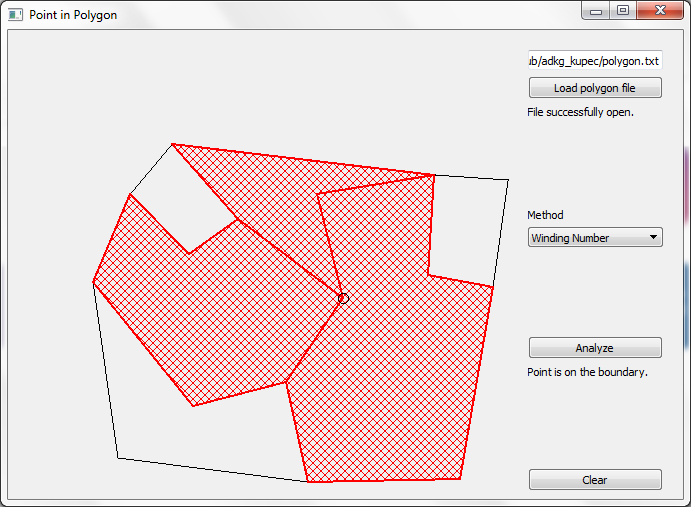
\includegraphics[width=13cm]{./pictures/gui_winding.png}
	%\caption{Výstup při použití \textit{Winding Number Algorithm} pro $q$ ležící ve více vrcholech polygonů}
%\end{figure}

\clearpage
 
\section{!Dokumentace}
Tato kapitola obsahuje dokumentaci k jednotlivým třídám.

\subsection{Algorithms}
Třída \textit{Algorithms} obsahuje tři základní metody, které nad vstupní množinou bodů vytváří konvexní obálky. Dále obsahuje pomocné metody k výpočtu úhlu mezi dvěma přímkami a metody k určování vztahu bodu a přímky.

\subsubsection{CHJarvis}
Metoda \textbf{CHJarvis} vytváří konvexní obálku obálku nad vstupní množinou bodů za použití algoritmu \textit{Jarvis Scan}. Na vstupu je vektor bodů třídy \texttt{QPoint}. Návratová hodnota je polygon třídy \texttt{QPolygon}, který obsahuje uspořádané body tvořící konvexní obálku.\\

\textbf{Input}:
\begin{itemize}
\item \textsl{vector} $\textless$\texttt{QPoint}$\textgreater$ $points$
\end{itemize}

\textbf{Output}:
\begin{itemize}
\item \texttt{QPolygon}
\end{itemize}

\subsubsection{QHull}
Metoda \textbf{QHull} vytváří konvexní obálku obálku nad vstupní množinou bodů za použití algoritmu \textit{Quick Hull}. Na vstupu je vektor bodů třídy \texttt{QPoint}. Návratová hodnota je polygon třídy \texttt{QPolygon}, který obsahuje uspořádané body tvořící konvexní obálku.\\

\textbf{Input}:
\begin{itemize}
\item \textsl{vector} $\textless$\texttt{QPoint}$\textgreater$ $points$
\end{itemize}

\textbf{Output}:
\begin{itemize}
\item \texttt{QPolygon}
\end{itemize}

\subsubsection{qh\_loc}
Metoda \textbf{qh\_loc} je lokální procedura algoritmu \textbf{QHull}, která se volá rekurzivně a hledá nejvzdálenější bod od přímky v dané polorovině a přidává jej do konvexní obálky poloroviny $H_i$. Na vstupu jsou dvě proměnné typu \texttt{int}, které obsahují index počátečního ($s$) a koncového bodu ($e$) dané přímky, vektor bodů vstupní poloroviny třídy \texttt{QPoint} a polygon třídy \texttt{QPolygon}, ve kterém jsou uloženy body konvexní obálky. Návratová hodnota je typu \texttt{void}.\\

\textbf{Input}:
\begin{itemize}
\item \texttt{int} $s$
\item \texttt{int} $e$
\item \textsl{vector} $\textless$\texttt{QPoint}$\textgreater$ $ss$
\item \texttt{QPolygon} $h$
\end{itemize}

\subsubsection{CHSweepLine}
Metoda \textbf{CHSweepLine} vytváří konvexní obálku obálku nad vstupní množinou bodů za použití algoritmu \textit{Sweep Line}. Na vstupu je vektor bodů třídy \texttt{QPoint}. Návratová hodnota je polygon třídy \texttt{QPolygon}, který obsahuje uspořádané body tvořící konvexní obálku.\\

\textbf{Input}:
\begin{itemize}
\item \textit{vector}<\texttt{QPoint}> $points$
\end{itemize}

\textbf{Output}:
\begin{itemize}
\item \texttt{QPolygon}
\end{itemize}

\subsubsection{get2LinesAngle}
Metoda \textbf{get2LinesAngle} počítá úhel mezi dvěma přímkami. Na vstupu jsou 4 body typu \texttt{QPoint}, návratová hodnota typu \texttt{double} vrací velikost úhlu v radiánech. Body $p_1$ a $p_2$ definují první přímku, zbylé dva body druhou přímku.\\

\textbf{Input}:
\begin{itemize}
\item \texttt{QPoint} $p_1$ 
\item \texttt{QPoint} $p_2$ 
\item \texttt{QPoint} $p_3$
\item \texttt{QPoint} $p_4$
\end{itemize}

\textbf{Output}:
\begin{itemize}
\item \texttt{double} 
\end{itemize}

\subsubsection{getPointLineDistance}
Metoda \textbf{getPointLineDistance} počítá nejkratší (kolmou) vzdálenost bodu $q$ od přímky tvořené dvěma body. Na vstupu jsou 3 body typu \texttt{QPoint}, návratová hodnota typu \texttt{double} vrací vzdálenost bodu $q$ od přímky.\\ 

\textbf{Input}:
\begin{itemize}
\item \texttt{QPoint} $q$ 
\item \texttt{QPoint} $a$ 
\item \texttt{QPoint} $b$
\end{itemize}

\textbf{Output}:
\begin{itemize}
\item \texttt{double} 
\end{itemize}

\subsubsection{getPointLinePosition}
Metoda \textbf{getPointLinePosition} určuje polohu bodu $q$ vzhledem k přímce tvořené dvěma body. Na vstupu jsou 3 body typu \texttt{QPoint}, návratová hodnota je nově definovaný typ \texttt{TPosition}.\\

\textbf{Input}:
\begin{itemize}
\item \texttt{QPoint} $q$
\item \texttt{QPoint} $a$
\item \texttt{QPoint} $b$
\end{itemize}

\textbf{Output}:
\begin{itemize}
\item \texttt{LEFT} $\rightarrow$ bod se nachází vlevo od přímky
\item \texttt{RIGHT} $\rightarrow$ bod se nachází vpravo od přímky
\item \texttt{ON} $\rightarrow$ bod se nachází na přímce
\end{itemize}

\subsection{Draw}
Třída \textit{Draw} obsahuje metody, které slouží ke generaci vstupní množiny bodů a k jejímu vykreslení. Dále vykresluje konvexní obálku dané množiny. 

\subsubsection{!paintEvent}
Metoda \textbf{paintEvent} vykresluje polygony a analyzovaný bod $q$. Návratová hodnota je typu \textit{void}.

\textbf{Input}:
\begin{itemize}
\item QPaintEvent *e
\end{itemize}

\subsubsection{!mousePressEvent}
Metoda \textbf{mousePressEvent} slouží k načtení souřadnic bodu $q$. Návratová hodnota je typu \textit{void}.

\textbf{Input}:
\begin{itemize}
\item QMouseEvent *e
\end{itemize}

\subsubsection{!clearAll}
Metoda \textbf{clearCanvas} slouží k vymazání všech vykreslených dat. Metoda neobsahuje žádné proměnné na vstupu a návratová hodnota je typu \textit{void}.

\subsubsection{!fillPolygon}
Metoda \textbf{fillPolygon} barevně vyšrafuje polygon, ve kterém se nachází analyzovaný bod $q$. Návratová hodnota je typu \textit{void}.

\textbf{Input}:
\begin{itemize}
\item $std::vector\textless std::vector\textless QPoint\textgreater \textgreater$ poly\_fill
\end{itemize}

\subsubsection{!loadPolygon}
Metoda \textbf{loadPolygon} slouží k nahrání bodů jednotlivých polygonů do aplikace. Součástí metody je i kontrola, zda se soubor úspěšně nahrál, zda vůbec obsahuje nějaké polygony a zda jsou polygony tvořeny aspoň 3 body. Návratová hodnota je typu \textit{QString} vrací hlášku, zda byly polygony úspěšně nahrány.

\textbf{Input}:
\begin{itemize}
\item const char* path
\end{itemize}

\textbf{Output}:
\begin{itemize}
\item QString
\end{itemize}

\subsection{SortByXAsc}
Třída obsahuje jedinou metodu(??konstruktor) \textbf{SortByXAsc}, která má na vstupu dva body typu \texttt{QPoint}, návratová hodnota je typu \texttt{bool}. Metoda vrací bod s nižší  souřadnicí X. Mají-li oba body shodnou souřadnici X, vrací bod s nižší souřadnicí Y.\\

\textbf{Input}:
\begin{itemize}
\item \texttt{QPoint} $p_1$
\item \texttt{QPoint} $p_2$
\end{itemize}

\textbf{Output}:
\begin{itemize}
\item 0 $\rightarrow$ bod $p_2$ má nižší $x$ souřadnici
\item 1 $\rightarrow$ bod $p_1$ má nižší $x$ souřadnici
\end{itemize}

\subsection{SortByYAsc}
Třída obsahuje jedinou metodu(??konstruktor) \textbf{SortByYAsc}, která má na vstupu dva body typu \texttt{QPoint}, návratová hodnota je typu \texttt{bool}. Metoda vrací bod s nižší  souřadnicí Y. Mají-li oba body shodnou souřadnici Y, vrací bod s nižší souřadnicí X.\\

\textbf{Input}:
\begin{itemize}
\item \texttt{QPoint} $p_1$
\item \texttt{QPoint} $p_2$
\end{itemize}

\textbf{Output}:
\begin{itemize}
\item 0 $\rightarrow$ bod $p_2$ má nižší souřadnici Y
\item 1 $\rightarrow$ bod $p_1$ má nižší souřadnici Y
\end{itemize}

\subsection{!Widget}
Metody třídy \textbf{Widget} slouží pro práci uživatele s aplikací. Až na jednu výjimku nemají metody na vstupu nic, návratové hodnoty všech metod jsou typu \textit{void}.

\subsubsection{!writeResult}
Metoda \textbf{writeResult} vrací polohu bodu $q$ vzhledem k polygonu na základě vstupní hodnoty typu \textit{int}.\\

\textbf{Input}:
\begin{itemize}
\item int
\end{itemize}

\subsubsection{on\_ch\_button\_clicked}
Metoda \textbf{on\_ch\_button\_clicked} načítá data z textového formátu. Uživatel sám vyhledává cestu k požadovanému souboru.

\subsubsection{on\_clear\_button\_clicked}
Metoda \textbf{on\_clear\_button\_clicked} vrací aplikaci do výchozí polohy smazáním všeho, co bylo vykresleno. 

\clearpage
\section{!Závěr}
V rámci úlohy \textit{Geometrické vyhledávání bodu} byla vytvořena aplikace, která určuje polohu analyzovaného bodu $q$ vzhledem k polygonu. Z důvodu větší časové náročnosti úlohy než obě autorky původně očekávaly nebyly implementovány všechny bonusové úlohy a některé části kódu mohly být řešeny lépe. Tato opravená verze technické zprávy je aktualizována o několik vzorců a o text v sekci Zadání. 

Jedná se například o použití tříd QPoint a QPolygon, které na vstupu mají hodnoty typu \textit{int} a které mohly být nahrazeny třídami QPointF a QPolygonF, jež na vstupu mají hodnot typu \textit{float}, což je pro práci se souřadnicemi bodů praktičtější. Dále jako ne zrovna nejšťastnější řešení hodnotíme množství vstupních hodnot, které mají na vstupu metody \textit{getPointLinePosition}, \textit{getTwoVectorsAngle} a \textit{getDistanceEdgeQ} třídy \textbf{Algorithms}. Vhodné by bylo nahradit jednotlivé souřadnice třídou QPoint, resp. QPointF. 

Dále mohlo být implementováno více kontrolních podmínek pro načítání bodů polygonu z textového souboru, například ošetření, zda soubor neobsahuje text, zda všechny body mají $x$ a $y$ souřadnici apod. Umisťování bodu $q$ do hran či vrcholů polygonů vyžaduje notnou dávku trpělivosti, aby se zobrazil korektní výsledek. Experimentálně bylo zjištěno, že aplikace zvládá lépe (tzn. je potřeba méně pokusů na kliknutí) zobrazovat polohu bodu $q$ ve vrcholech než v hranách, ač obě situace jsou v kódu ošetřené. 

Úloha přinesla i pozitivní přínos v tom směru, že se autorky mohly potrénovat v psaní kódu v jazyce C++ a oprášit své znalosti psaní v prostředí LaTeX.

\clearpage

\section{Zdroje}
\begin{enumerate}
\item  \textsl{BAYER, Tomáš. Geometrické vyhledávání bodů} [online][cit. 24. 10. 2018].\\
Dostupné z: \href{https://web.natur.cuni.cz/~bayertom/images/courses/Adk/adk4.pdf}{https://web.natur.cuni.cz}

\item  \textsl{CS 312 - Convex Hull Project} [online][cit. 10. 11. 2018].\\
Dostupné z: \href{http://mind.cs.byu.edu/courses/312/projects/project2_files/ConvexHull_python.php}{http://mind.cs.byu.edu}

\item  \textsl{SOPUCH, Pavel. LaTeX v kostce} [online][cit. 12. 11. 2018].\\
Dostupné z: \href{http://www.it.cas.cz/manual/latex/}{http://www.it.cas.cz}


\end{enumerate}
\end{document}

%polomer kruznice dan predem -> omezeni aby body nevylezly z platna
%chybova hlaska, zadame-li vic bod nez je mozne
%defaultní vstupní data